\documentclass[soumission]{ir}

\titre{Initiation à la recherche \\Classification de musique non supervisée}

\auteur{Lafille Julien et Ouali Kouceilal}

\titrecourt{Classification de musique non supervisée}

\nomcourt{J. Lafille et K. Oualil}

\encadrant{Alexendre Blansché}

\motcle{Annalyse de signal, Musique, Classification, Non supervisé}

\begin{document}

\section{Introduction}

\section{Etat de l'art}
La musique étant massivement présente en format numérique, et le besoin de classer les différentes musiques
 étant toujours aussi présent, les chercheurs ont développé différentes techniques permettant d’automatiser 
 le processus.

\subsection{L’analyse et la classification musicale}
\paragraph{}
La recommandation de musique s’appuie essentiellement sur l’identification des genres. L’humain étant capable 
de reconnaître un genre musical dans 70\% des cas au bout de 3 secondes d’écoutes seulement, et dans 50\% 
des cas au bout de 0.25 secondes \cite{TechniqueSimilarites}, les chercheurs ont essayé de réaliser cette 
discrimination de manière automatique et se sont reposés sur l’analyse et l’extraction des données physiques 
des fichiers audio. Ainsi, les critères formels pris en compte ont été utilisés pour différencier les divers 
genres musicaux et attribuer chaque titre à l’un de ces genres.
\paragraph{}
La difficulté réside dans le choix de critères pertinents, divers techniques se sont développées au fil du 
temps et les chercheurs se sont notamment basés sur la structure rythmique, la superposition des instruments, 
ou encore le timbre. Deux approches sont particulièrement utilisées dans le domaine, la première se repose 
sur l’analyse du signal, qui utilise la reconnaissance de motifs et la construction d’une “surface musicale” 
\cite{TechniqueSimilarites} et la seconde sur l'analyse des caractéristiques physiques de haut niveau se 
basant sur l’analyse de partitions musicales (qui permet d’extraire des données telle que la hauteur d’une 
note), cette dernière technique étant possible même quand le fichier audio n’est pas disponible.

\subsection{Les systèmes de recommandation}
\paragraph{}
Souvent dans le but de fidéliser l’utilisateur et maximiser le temps qu’il passe sur la plateforme, les 
systèmes de recommandation (que ce soit celles utilisées par les plateformes de streaming audio comme Deezer 
et Spotify, vidéo comme Youtube et les réseaux sociaux comme Facebook) utilisent les données récoltées au 
cours de l’utilisation du service par un profil utilisateur pour affiner les recommandations en plus des 
autres techniques de classements.

\paragraph{}
Une analyse contextuelle est bien souvent nécessaire pour avoir des résultats plus proches de la sensibilité 
humaine, en prenant en compte les subjectivités liées à la reconnaissance de genres par l’Homme (comme les 
influences culturelles ou l’émotion). Cette analyse se fait souvent sur les métadonnées récoltées en continu 
et qui évoluent en suivant les tendances. Pour cela, ils se basent sur l’utilisateur en lui-même et ses 
interactions (autant avec les items qu’avec les autres utilisateurs). On utilise les deux approches, souvent 
complémentaires, qui sont : 
\begin{itemize}
    \item{Le filtrage par contenu, s'intéressant au couple \textit{[Profil utilisateur-Item]} et sur l’appréciation 
    de l’utilisateur concernant cet item. La proximité des items est affinée en recueillant ces appréciations 
    et l’utilisateur se voit recommander les items les plus pertinents en vue de sa notation ou de son 
    nombre de consultations des items voisins.}
    \\
    \item{Le filtrage collaboratif, quant à lui, crée une proximité sociale entre les utilisateurs et classe 
    les items selon les affinités entre utilisateurs afin de proposer un item “populaire” au sein d’un 
    groupe aux utilisateurs en faisant partie.}
\end{itemize}

\paragraph{}
Mais c’est généralement des méthodes hybrides qui sont utilisées dans les services de recommandation. Ces 
données sont exploitées par des algorithmes de classification supervisés en se reposant sur les classements 
faits par les libraires, les radios et les musicologues pour les caractéristiques liées aux musiques et sur 
les données récoltées lors de l’utilisation du service par l’utilisateur pour ce qui est des métadonnées. 
Mais les différentes subjectivités et les définitions parfois très vagues de certains genres sont une source 
importante d’erreurs. De plus, l’analyse contextuelle favorise l’enfermement de l’auditeur dans un univers 
restreint et peine à réellement recommander de nouveaux genres, s’ajoute à cela qu’en prenant en compte la 
popularité des morceaux, en cas de filtrage collaboratif, il est moins probable que ces techniques 
recommandent un titre impopulaire mais proche des goûts musicaux de l’auditeur (qu’il serait donc 
susceptible d'apprécier).

\subsection{Propositions}
\paragraph{}
Les techniques énoncées précédemments se basent sur un mimétisme des choix des utilisateurs et sur les 
étiquetages et ne se reposent pas sur une classification objective de la musique. De ce fait, il est plus 
difficile de classifier les genres de manière universelle. Nous nous proposons donc de chercher un moyen de 
classer la musique de façon plus indépendante de l’utilisateur dans un premier temps, mais aussi de façon 
indépendante des genre déjà définis, et ce pour plusieurs raisons :
\begin{itemize}
    \item {Il n’y a pas de réel consensus sur une liste exhaustive de genres musicaux.}
    \item {La définition de certains genres musicaux étant floue et assez vague pour comprendre une même 
    chanson dans plusieurs genres.}
    \item {Ils sont basés sur des influences culturelles et parfois ancrées dans un air temporel défini.}
\end{itemize}

\paragraph{}
Une fois que le classement ait été établi grâce à des algorithmes de classification non supervisée (qui se 
baseront donc essentiellement sur l’analyse musicale), nous intégrerons les préférences de l’auditeur au 
modèle pour isoler et pouvoir proposer les items les plus proches de ses envies. Cette classification 
indépendante des constructions “artificielles” de catégories de musiques est susceptible de rassembler les 
items dans des groupes aux frontières potentiellement mieux définies.

\section{Analyse audio}
\paragraph{}
Les algorithmes de clustering ont besoin de données pour effectuer une classification. Nos données initiales 
sont des fichiers audio, ils contiennent le signal musical en lui-même et quelques métadonnées telles que le 
titre, l’artiste ou encore l'album. Nous voulions dans notre démarche proposer des chansons similaires sans 
se baser sur les métadonnées des chansons, mais plutôt la similitude des chansons. La seule métadonnée que 
nous utiliserons est donc la durée.

\paragraph{}
Il n’est pas possible de donner aux algorithmes de clustering directement le signal, nous devons donc 
“simplifier” le signal en données exploitables pour ces algorithmes. Beaucoup de travaux ont été réalisés 
en analyse de musique et analyse vocale. Un grand nombre de ces travaux se base sur l’analyse du signal 
audio. Certains critères calculables à partir du signal sont assez récurrents dans les différents travaux 
du domaine, c’est pourquoi nous avons décidé de les utiliser comme critères pour effectuer notre 
classification.

\subsection{Présentation des données}
\paragraph{}
Nous avons retenu 4 critères assez communs en analyse audio que nous allons détailler dans cette section : 
le Zero Crossing Rate, le Root Mean Square, la Centroid et le Spread. Nous devons déjà expliquer la nature 
de nos données.

\paragraph{}
Un signal audio analogique peut être vu comme la pression exercée par une source sur l’air qui l’entoure 
dans le temps. Cette pression de l’air est captée par nos oreilles ou bien un microphone. Sa nature est 
continue, pour transformer ce signal continu en information on utiliser une méthode d'échantillonnage pour 
discrétiser l’information, on a alors un signal numérique.

\begin{figure}
    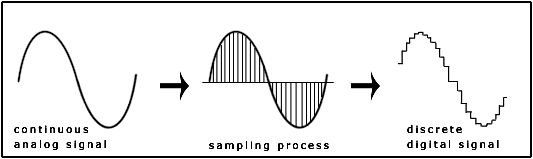
\includegraphics[scale=0.7]{images/Sampling-of-audio-signal.png}
    \caption{Echantillonage d'un signal continu}
\end{figure}

\paragraph{}
La fréquence d'échantillonnage (Fe) détermine la fréquence à laquelle chaque échantillon est pris. Plus la 
fréquence est haute plus le signal numérique est proche du signal analogique. Le sampling mène à une  perte 
d’information s’il existe des variations plus rapides que la fréquence d'échantillonnage. De manière 
générale on dit que le signal est bien représenté tant qu’il ne contient pas une fréquence supérieure à 
$\frac{Fe}{2}$. C’est pourquoi le standard dans l’industrie de la musique est \textit{Fe = 44100 Hz} ce qui 
permet de couvrir tout le spectre de l’audition humaine ( 20 Hz à 20000 Hz) avec un peu de marge.

\paragraph{}
Une chanson contient en général deux pistes audio pour donner un effet stéréo. Nous convertissons ces deux pistes 
stéréo en une seule piste mono pour conduire nos analyses. Nous découpons ensuite le signal en morceaux plus
 courts pour calculer chacun de nos critères en gardant l’aspect temporel de la musique. Nous avons choisit 
 de découper le signal en sections de une seconde, qui est un bon compromis entre vitesses de calcul des 
 critères et précision temporelle \cite{Survey}.

\subsection{Critères temporels}
\paragraph{}
Nous pouvons maintenant calculer deux de nos critères, le premier étant le zero crossing rate, ou taux de 
passage par zéro. Ce critère permet d’avoir une estimation du timbre du signal (un signal aigu passera par 
zéro plus fréquemment qu’un signal grave).
\begin{equation}
    ZCR = \frac{1}{N}*\sum_{n = 1}^{N} \delta( x_{n-1}*x_n \leqslant 0 )
\end{equation}

\noindent{Avec $x_i$ le i-ème echantillon du signal, $N$ le nombre d'échantillons et : }\\

$\delta(x)=\begin{cases}
    1, & \text{si $x$ est vrai}.\\
    0, & \text{sinon}.
\end{cases}$

\paragraph{}
Le second critère est le root mean square : ce critère permet de calculer l'énergie moyenne du signal sur une période.
\begin{equation}
    RMS = \sqrt{\frac{1}{N}*\sum_{n = 0}^{N} x_n^2}
\end{equation}

\subsection{Critères fréquentiels}

\section{Classification}

\subsection{Méthodes adoptées}

\subsection{Mise en oeuvre}

\section{Résultat expérimentaux}

\subsection{Protocole}

\subsection{Resultats}

\section{Conclusion}


\bibliographystyle{apalike}
\bibliography{IR_biblio}

\appendix

\end{document}
